% Created 2019-11-05 mar. 17:28
% Intended LaTeX compiler: pdflatex
\documentclass[t]{clean-beamer}
\usepackage[utf8]{inputenc}
\usepackage[T1]{fontenc}
\usepackage{graphicx}
\usepackage{grffile}
\usepackage{longtable}
\usepackage{wrapfig}
\usepackage{rotating}
\usepackage[normalem]{ulem}
\usepackage{amsmath}
\usepackage{textcomp}
\usepackage{amssymb}
\usepackage{capt-of}
\usepackage{hyperref}
\usepackage[most]{tcolorbox}
\usepackage{siunitx}
\beamertemplatenavigationsymbolsempty
\addtobeamertemplate{navigation symbols}{}{%
\usebeamerfont{footline}%
\usebeamercolor[fg]{footline}%
\hspace{1em}%
\insertframenumber/\inserttotalframenumber
}
\setbeamertemplate{itemize items}[circle]
\usefonttheme[onlymath]{serif}
\usetheme{default}
\author{Dehaeze Thomas\textsuperscript{$\dagger$} \\ Vermat Mohit \\ Collette Christophe \\ \vspace{1cm} 08-11-2019 \\ \vspace{1cm} \textsuperscript{$\dagger$} Email: {\tt\small thomas.dehaeze@esrf.fr}}
\date{}
\title{Complementary Filters Shaping\newline Using \(\mathcal{H}_\infty\) Synthesis}
\subtitle{ICCMA 2019}
\begin{document}

\maketitle

\begin{frame}[label={sec:org3efdf18}]{Sensor Fusion}
In order to improve the estimate \(\hat{x}\) of \(x\), multiple sensors can be merged together using complementary filters.

This permits to have

High bandwidth
\begin{itemize}
\item need of Sensor at low frequency + sensor at high frequency
\item need of merging the two
\item complementary filters
\item design of those filters using \(\mathcal{H}_\infty\)
\end{itemize}

Goal:
\begin{itemize}
\item Higher control bandwidth
\item Better estimation of some physical value
\end{itemize}

Applications:
\begin{itemize}
\item LIGO - Vibration isolation of precise equipment
\item UAV - Angle estimation using Accelerometer and Gyroscope
\end{itemize}
\end{frame}

\begin{frame}[label={sec:org132896d}]{Sensor Fusion Architecture - Noise Filtering}
\vspace{-1em}
\begin{columns}
\begin{column}{0.45\columnwidth}
\vspace{-1em}
\begin{center}
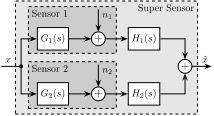
\includegraphics[scale=1,width=1.1\linewidth]{figs/fusion_super_sensor.pdf}
\end{center}
\end{column}

\begin{column}{0.55\columnwidth}
\begin{equation*}
  \hat{x} = \left(G_1 H_1 + G_2 H_2\right) x + H_1 n_1 + H_2 n_2
\end{equation*}

\onslide{\begin{cbox}[Complementary Property]{blue}{}
\begin{equation*}
  H_1(s) + H_2(s) = 1
\end{equation*}
\end{cbox}}\vspace{0.5em}
\end{column}
\end{columns}

\vspace{0.5em}
Let's first consider \textbf{Perfectly Known Sensor Dynamics}:
\begin{equation*}
  G_1(s) = G_2(s) = 1 \Longrightarrow \tcmbox{\hat{x} = x + H_1 n_1 + H_2 n_2}
\end{equation*}

\onslide{\begin{cbox}[PSD of the Super Sensor's noise]{blue}{ams nodisplayskip}
\begin{equation*}
  \Phi_{\hat{x}} = \left|H_1\right|^2 \Phi_{n_1} + \left|H_2\right|^2 \Phi_{n_2} \Longrightarrow \text{depends on filters' norm}
\end{equation*}
\end{cbox}}\vspace{0.5em}
\end{frame}


\begin{frame}[label={sec:orgcb2d144}]{Shaping of Complementary Filters using \(\mathcal{H}_\infty\) synthesis}
\vspace{-1em}
\begin{columns}
\begin{column}{0.5\columnwidth}
\onslide{\begin{cbox}[Design Objective]{blue}{ams nodisplayskip}
\begin{gather*}
  H_1(s) + H_2(s) = 1 \\
  |H_1(j\omega)| \le \frac{1}{|W_1(j\omega)|} \quad \forall\omega \\
  |H_2(j\omega)| \le \frac{1}{|W_2(j\omega)|} \quad \forall\omega
\end{gather*}
\end{cbox}}\vspace{0.5em}

\onslide{\begin{cbox}[]{blue}{}
\(W_1(s)\) and \(W_2(s)\) are proper, stable and minimum phase transfer functions
\end{cbox}}\vspace{0.5em}
\end{column}

\begin{column}{0.5\columnwidth}
\vspace{-3em}
\begin{center}
\includegraphics[scale=1,width=\linewidth]{figs/h_infinity_robust_fusion.pdf}
\end{center}

\onslide{\begin{cbox}[\(\mathcal{H}_\infty\) Synthesis]{blue}{}
Find \(H_2(s)\) such that:
\begin{gather*}
  \left\|\begin{matrix} \left[1 - H_2(s)\right] W_1(s) \\ H_2(s) W_2(s) \end{matrix}\right\|_\infty \le 1 \\
  H_1(s) \triangleq 1 - H_2(s)
\end{gather*}
\end{cbox}}\vspace{0.5em}
\end{column}
\end{columns}
\end{frame}

\begin{frame}[label={sec:orgff066bd}]{Validation of the proposed synthesis method}
\begin{figure}[htbp]
\centering
\includegraphics[scale=1]{figs/hinf_synthesis_results.pdf}
\caption{\label{fig:hinf_synthesis_results}
Frequency response of the weighting functions and complementary filters obtained using \(\mathcal{H}_\infty\) synthesis}
\end{figure}
\end{frame}

\begin{frame}[label={sec:org92cdf48}]{\(\mathcal{H}_\infty\) Synthesis of Complementary filters used at LIGO}
\begin{figure}[htbp]
\centering
\includegraphics[scale=1]{figs/comp_fir_ligo_hinf.pdf}
\caption{\label{fig:comp_fir_ligo_hinf}
Comparison of the FIR filters (solid) designed at LIGO with the filters obtained with \(\mathcal{H}_\infty\) synthesis (dashed)}
\end{figure}
\end{frame}
\end{document}